%!TEX root = ../thesis_a4.tex

\chapter{\titlecap{Automatic \glsentrytext{raga} Recognition}}


%0) What is automatic raga identification
%1) Motivation and relevance of the problem
%2) References to thousands of papers that cater to this task
%3) What lacks in them
%4) How do we fill in the missing gaps
%5) What we present in this chapter
%6) What are the papers which this chapter is based on


\section{Introduction}

In this chapter we address the task of automatic \gls{raga} recognition, which is one of the most studied topics within \gls{mir} of Indian art music. We begin by highlighting the shortcomings of the existing \gls{raga} recognition approaches and subsequently present two different methods to address these limitations. We evaluate the proposed methods on representative and sizable collection of Hindustani and Carnatic music, both of which are made publicly available. In addition to evaluating our proposed methods we also compare their performance with the state of the art approaches by evaluating them under the same experimental conditions for the same data set.  

\TODO{Do we need to write what is automatic raga recognition?}

As mentioned before \gls{raga} is a core musical concept used in the composition, performance, organization, and pedagogy of Indian art music (IAM). Numerous compositions in Indian folk and film music are also based on \glspl{raga}~\citep{ganti2013bollywood}. Despite its significance in IAM, there exists a large volume of audio content whose \gls{raga} is incorrectly labeled or, simply, unlabeled. This is partially because the vast majority of the tools and technologies that interact with the recordings' metadata fall short of fulfilling the specific needs of the Indian music tradition~\citep{XavierSerra2011}. A computational approach to automatic \gls{raga} recognition can enable \gls{raga}-based music retrieval from large audio collections, semantically-meaningful music discovery, musicologically-informed navigation, as well as several applications around music pedagogy. 

\Gls{raga} recognition as mentioned earlier is widely studied topics within \gls{mir} of IAM. As a consequence, there exist a considerable amount of approaches utilizing different characteristic aspects of \glspl{raga}. A summary of these approaches is already provided in Section XXX. A large number of approaches for \gls{raga} recognition use features derived from the pitch or pitch-class distribution as can be seen in Table~XXXX. Using these features they capture the overall usage of the tonal material in an audio recording. In general, PCD-based approaches are robust to pitch octave errors, which is one of the most frequent errors in the estimation of predominant melody from polyphonic music signals. Currently, the PCD-based approach represents the state-of-the-art in \gls{raga} recognition~\citep{chordia2013joint}. Along with the merits there are several limitations of the these approaches. One of the major shortcomings of the PCD-based approaches is that they completely disregard the temporal aspects of the melody, which are essential to \gls{raga} characterization~\cite{rao1999raga}. Temporal aspects are even more relevant in distinguishing phrase-based \glspl{raga}~\cite{krishna2012carnatic}, as their aesthetics and identity is largely defined by the usage of meandering melodic movements, called gamakas. 

Several approaches address this shortcoming in the PCD-based approaches by modeling the temporal aspects of a melody in a variety of ways~\cite{kumar2014identifying, shetty2009raga, rajkumar2011identification}. Such approaches typically use melodic progression templates~\cite{shetty2009raga}, n-gram distributions~\cite{kumar2014identifying}, or hidden Markov models~\cite{rajkumar2011identification} to capture the sequential information in the melody. With that, they primarily utilize the \={a}r\={o}hana-avr\={o}hana pattern of a \gls{raga}. In addition, most of them either transcribe the predominant melody in terms of a discrete svara sequence, or use only a single symbol/state per svara. Thus, they discard the characteristic melodic transitions between svaras, which are a representative and distinguishing aspect of a \gls{raga}~\cite{rao1999raga}. Furthermore, they often rely on an accurate transcription of the melody, which is still a challenging and an ill-defined task given the nature of IAM~\cite{rao2012culture, Suvarnalata2014}. 

As mentioned before melodic patterns are one of the most prominent cues for \gls{raga} identification, used both by a performer and a listener~\citep{rao1999raga}. Despite the importance there do not exist many approaches that exploit these patterns for automatic \gls{raga} recognition. This can be attributed to the challenges involved in the extraction of characteristic melodic phrases in audio music collections. To the best of our knowledge there exist only two approaches so far that use melodic patterns for this task~\cite{shrey_ISMIR_2015, sridhar2009raga}, out of which only the former considers a continuous melodic contour for melodic phrases. Their aim is to create dictionaries of characteristic melodic phrases and to utilize them in the recognition phase. \TODO{What are the critical remarks for these two approaches?}

\begin{figure}
	\begin{center}
		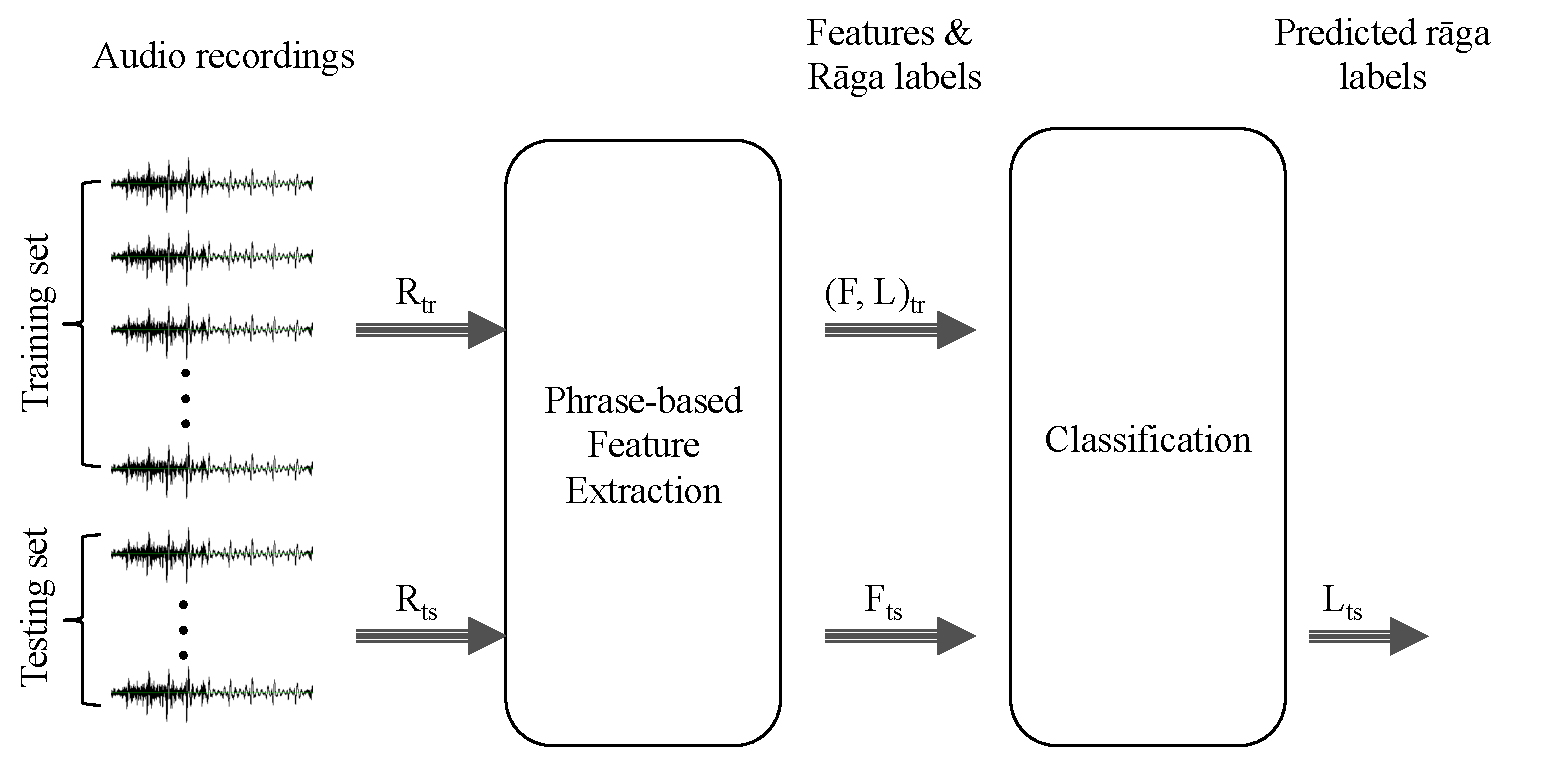
\includegraphics[width=\figSizeHundred]{ch07_ragaRecognition/figures/bd_overall_phasebased_raga_recognition.pdf}
	\end{center}
	\caption{Overall block diagram for automatic \gls{raga} recognition.}
	\label{fig:bd_raga_recognition}
\end{figure}



In this chapter we describe two novel methods $\mathcal{M}_\mathrm{\acrshort{vsm}}$~\TODO{Citations for both} and $\mathcal{M}_\mathrm{\acrshort{tdms}}$ that overcome a number of shortcomings in the existing approaches described above and improve the accuracy of \gls{raga} recognition. A general block diagram for both the methods is shown in Figure~\ref{fig:bd_raga_recognition}. There are two main processing blocks; feature extraction and classification. Given sets of audio recordings for training ($\mathrm{R}_\mathrm{tr}$) and testing ($\mathrm{R}_\mathrm{ts}$) we first extract features ($\mathrm{F}_\mathrm{tr}$ and $\mathrm{F}_\mathrm{ts}$) for every audio recording in both the sets. Subsequently features of the training set $\mathrm{F}_\mathrm{tr}$ along with the \gls{raga} labels $\mathrm{L}_\mathrm{tr}$ are used to train a classifier to build a classification model. Using this model we then predict the \gls{raga} labels for the testing set $\mathrm{L}_\mathrm{ts}$. $\mathcal{M}_\mathrm{\acrshort{vsm}}$ and $\mathcal{M}_\mathrm{\acrshort{tdms}}$ differ both in terms of the extracted features and the classification strategy. Both these methods are described at length in subsequent sections.


\section{\titlecap{Vector Space Modeling for \glsentrytext{raga} Recognition}}
\label{sec:phrase_based_feature_extraction}

A number of similarities can be seen between a \gls{raga} rendition and a textual description of a topic. Like an author describes a topic by using different relevant words to the topic, an artist renders a \gls{raga} by using appropriate melodic phrases that suit the context. There are words that are quite specific to a topic, which are analogous to the characteristic melodic phrases of a \gls{raga}. Stop words not specific to any topic or to a document can be seen as analogous to the generic gamaka type melodic patterns (for example, Kampita\footnote{a specific type of an oscillatory melodic movement on a svara~\cite{krishna2012carnatic}.}), which are not specific to a \gls{raga} or to a recording. Words that are specific to a document can be regarded as composition specific melodic patterns. This analogy drives the proposed method, which we denote by $\mathcal{M}_\mathrm{\acrshort{vsm}}$. $\mathcal{M}_\mathrm{\acrshort{vsm}}$ uses automatically discovered melodic patterns and employs concepts of \gls{vsm}. As can be imagined, the overall approach is inspired by the approaches typically used for topic modeling and document classification~\TODO{refs}.

Merits and shortcomings of this method are summarized below:
\begin{itemize}
	\item Human interpretation of the intermediate output, usability of intermediate outputs, exploiting the most characteristic aspect of a raga. Utilize both the tonal and the pitch information. Exploit characteristic movements between the svaras as well as sequence of svaras
	\item No need for analyzing whole melody, if patterns are identified in chunks raga can be identified.
	\item Musically meaningful relatinos between recordings can be established.
\end{itemize}

Cons
\begin{itemize}
	\item Prone to octave errors, not statistical, spurts of error can deprove the performance enormously
	\item Extraction of characteristic melodic patterns is still a challenging process. Limited by that performance
	\item Affected a lot by the improvisational aspects
	\item Computatinoally challenging. 
	\item Does not exploit global melodic characteristics.
\end{itemize}


\begin{figure}
	\begin{center}
		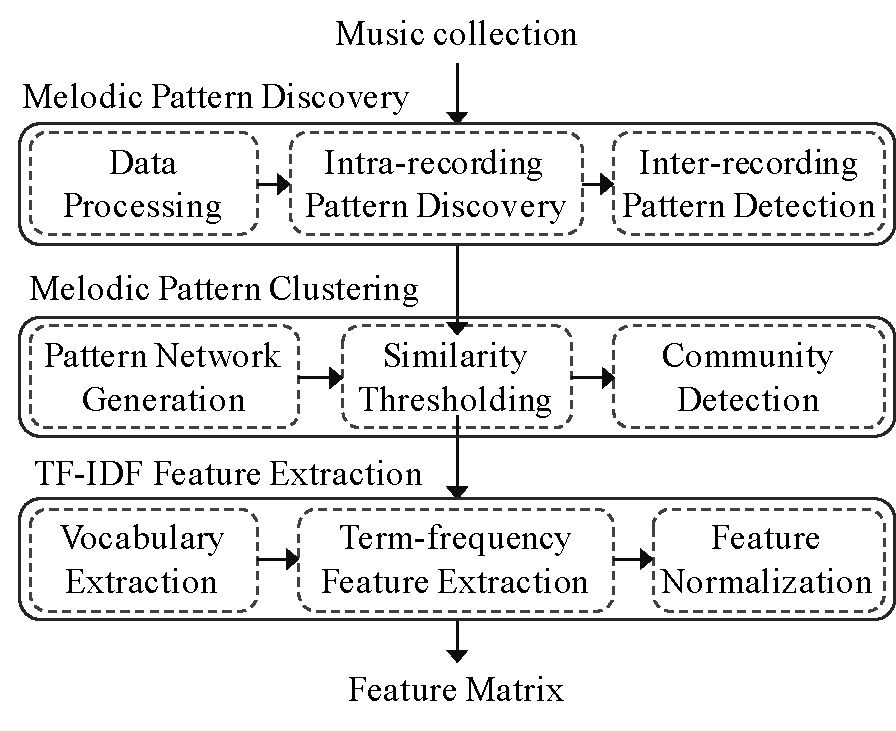
\includegraphics[width=\figSizeSeventy]{ch07_ragaRecognition/figures/bd_phasebased_raga_recognition.pdf}
	\end{center}
	\caption{Block diagram of the proposed phrase-based approach to \gls{raga} recognition.}
	\label{fig:bd_phasebased_raga_recognition}
\end{figure}




%In melodic pattern discovery block we follow an unsupervised approach and extract melodic patterns from audio music recordings. For this, we employ our proposed method for mining melodic patterns as described in Section~XXX that scales upto hundreds of hours of music data. These patterns are then clustered together into communities using the method described in Section~XXX. The occurrences of the melodic patterns clustered within communities are used to compute feature vector for each audio recording, which is eventually used for \gls{raga} classification.


\subsection{Feature Extraction}
\label{sec:vsm_feature_extraction}

The block diagram for feature extraction in $\mathcal{M}_\mathrm{\acrshort{vsm}}$ is shown in Figure~\ref{fig:bd_phasebased_raga_recognition}. There are three main processing blocks; melodic pattern discovery, melodic pattern clustering and feature extraction. Below we describe each of these blocks in detail. 

\subsubsection{Melodic Pattern Discovery}
\label{sec:vsm_feature_extraction_pattern_discovery}
In this block we extract melodic patterns from the collection of audio recordings. There are three main processing modules in this block; data-processing, intra-recording pattern discovery and inter-recording pattern search. All these modules are same as described already in Section~XXX. We use the same set of parameter settings as mentioned in their description.

\subsubsection{Melodic Pattern Clustering}
\label{sec:vsm_feature_extraction_pattern_clustering}

In this block we cluster the discovered melodic patterns obtained in the previous step. The objective is to group together all the patterns that are different occurrences of the same melodic phrase. For this, we propose to perform a network analysis in which the clustering is performed using a non-overlapping community detection method. 

We start by building an undirected network $\mathcal{G}$ using the discovered patterns as the nodes of the network. We connect any two nodes only if the distance between them is below a similarity threshold $T_s$. Noticeably, this distance is computed using the same measure as used in the pattern discovery block (Section~XXXX). The weight of the edge, when it exists, is set to 1. Non-connected nodes are removed.

As mentioned before determining a meaningful similarity threshold in an unsupervised manner is a complex task. For estimating an optimal value of $T_s$ we follow the approach as described in Section~\TODO{XXX}. We compare the evolution of the clustering coefficient $C$ of the obtained network $\mathcal{G}$ with a randomized network $\mathcal{G}_r$ over different distance thresholds $T_s$. The randomized network $\mathcal{G}_r$ is obtained by swapping the edges between randomly selected pairs of nodes such that the degree of each node is preserved~\cite{maslov2002specificity}. The optimal threshold $T_{s}^\star$ is taken as the distance that maximizes the difference between the two clustering coefficients.  In Figure~\TODO{XXX}, we show $C(\mathcal{G})$, $C(\mathcal{G}_r)$ and $C(\mathcal{G})-C(\mathcal{G}_r)$ for different values of $T_{s}$, and mark the optimal threshold $T_{s}^\star$.

The next step of our approach (Figure~\ref{fig:bd_phasebased_raga_recognition}) groups similar melodic patterns as done in Section~\TODO{XXX}. To do so, we detect non-overlapping communities in the network of melodic patterns using the method proposed in~\cite{blondel2008fast}. This method is based on optimizing the modularity of the network and is parameter-free from the user's point of view. This method is capable of handling very large networks and has been extensively used in various applications~\cite{fortunato2010community}. We use its implementation available in networkX~\cite{hagberg-2008-exploring}, a Python language package for exploration and analysis of networks and network algorithms. Note that, from now on, the melodic patterns grouped within a community are regarded as the occurrences of a single melodic phrase. Thus, a community essentially represents a melodic phrase or motif.

\subsubsection{TFIDF Feature Extraction}
\label{sec:vsm_feature_extraction_TFID_computation}

As mentioned above, we draw an analogy between r\={a}ga rendition and textual description of a topic. Using this analogy we represent each audio recording using a vector space model. This process is divided into three blocks (Figure~\ref{fig:bd_phasebased_raga_recognition}).

We start by building our vocabulary $P$, which translates to selecting relevant communities (melodic phrases) for characterizing r\={a}gas. For this, we include all the detected communities except the ones that comprise patterns extracted from only a single audio recording. Such communities are analogous to the words that only occur within a document and, hence, are irrelevant for modeling a topic. The size of the obtained vocabulary $P$ corresponding to the optimal threshold mentioned above ($T_{s}^\star=9$) is XXX.

We experiment with three different sets of features $\mathrm{F_1}$, $\mathrm{F_2}$ and $\mathrm{F_3}$, which are similar to the term frequency-inverse document frequency features typically used in text information retrieval. We denote our corpus by $R$  comprising $N = |R|$ number of recordings. A melodic phrase and a recording is denoted by $p$ and $r$ , respectively

\begin{equation}
\mathrm{F_1}(p,r)= 
\begin{cases}
1				,& \text{if}~~f(p,r) > 0\\
0,              & \text{otherwise}
\end{cases}
\end{equation}
where, $f(p,r)$ denotes the raw frequency of occurrence of phrase $p$ in recording $r$. $\mathrm{F_1}$ only considers the presence or absence of a phrase in a recording. In order to investigate if the frequency of occurrence of melodic phrases is relevant for characterizing r\={a}gas, we take $\mathrm{F_2}(p,r) = f(p,r)$. As mentioned, the melodic phrases that occur across different r\={a}gas and in several recordings are futile for r\={a}ga recognition. Therefore, to reduce their effect in the feature vector we employ a weighting scheme, similar to the inverse document frequency ($\mathrm{idf}$) weighting in text retrieval.
\begin{equation}
\mathrm{F_3}(p,r) = f(p,r) \times \mathrm{irf}(p,R)
\end{equation}
\begin{equation}
\mathrm{irf}(p,R) = \log \left( \frac{N}{ |\lbrace r \in R: p \in r \rbrace|} \right)
\end{equation}
where, $|\lbrace r \in R: p \in r \rbrace|$ is the number of recordings where the melodic phrase p is present, that is $f(p,r)\neq 0$ for these recordings. 

The number of melodic patterns obtained from an audio recording tends to be proportional to the length of the recording. In order to reduce the affect of different recording lengths, we investigate two feature vector normalization techniques frequently used in text classification. In addition to using raw features vectors we experiment with $L_1$ and $L_2$ normalization~\cite{leopold2002text}.\TODO{A better reference}. 


\subsection{Classification and Evaluation Methodology}
\label{sec:classification_based_raga_recognition}

The features obtained above are used to train a classifier. In order to assess the relevance of these features for r\={a}ga recognition, we experiment with different algorithms exploiting diverse classification strategies~\cite{Hastie09BOOK}: Multinomial, Gaussian and Bernoulli naive Bayes (NBM, NBG and NBB, respectively), support vector machines with a linear and a radial basis function kernel, and with a stochastic gradient descent learning (SVML, SVMR and SGD, respectively), logistic regression (LR) and random forest (RF). We use the implementation of these classifiers available in scikit-learn toolkit~\cite{scikitlearn}, version 0.15.1. Since in this study, our focus is to extract a musically relevant set of features based on melodic phrases, we use the  default parameter settings for the classifiers available in scikit-learn. 

We use a stratified 12-fold cross-validation methodology for evaluations. The folds are generated such that every fold comprises equal number of feature instances per r\={a}ga. We repeat the entire experiment 20 times, and report the mean classification accuracy as the evaluation measure. In order to assess if the difference in the performance of any two methods is statistically significant, we use the Mann-Whitney U test~\cite{mann1947test} with $p=0.01$. In addition, to compensate for multiple comparisons, we apply the Holm-Bonferroni method~\cite{holm1979simple}. 


\subsection{Results and Discussion}
\label{sec:vsm_eval_results}


\begin{table}
	\tabcolsep=.18cm
	\centering
	\begin{tabular}{c|c|c|c c c c c}
		\hline
		db & Mtd & Ftr & NBM & NBB & LR & SVML & 1NN\tabularnewline
		\hline \hline 
		\multirow{5}{*}{\begin{turn}{90}DB10r\={a}ga\end{turn}} & \multirow{3}{*}{$M$} & $\mathrm{F_1}$ & 90.6 & 74 & 84.1 & 81.2 & -\tabularnewline
		
		&  & $\mathrm{F_2}$ & {\bf 91.7} & 73.8 & 84.8 & 81.2 & -\tabularnewline
		
		&  & $\mathrm{F_3}$ & 90.5 & 74.5 & 84.3 & 80.7 & -\tabularnewline
		\cline{2-8} 
		& \multirow{2}{*}{$S_1$} & $\mathrm{PCD}_{120}$ & - & - & - & - & 82.2\tabularnewline
		& & $\mathrm{PCD}_{full}$ & - & - & - & - & {\bf 89.5}\tabularnewline
		\cline{2-8} 
		& $S_2$ & $\mathrm{PD}_{param}$ & 37.9 & 11.2 & {\bf 70.1} & 65.7 & -\tabularnewline
		\hline \hline
		\multirow{5}{*}{\begin{turn}{90}DB40r\={a}ga\end{turn}} & \multirow{3}{*}{$M$} & $\mathrm{F_1}$ & 69.6 & 61.3 & 55.9 & 54.6 & -\tabularnewline
		
		&  & $\mathrm{F_2}$ & {\bf 69.6} & 61.7 & 55.7 & 54.3 & -\tabularnewline
		
		&  & $\mathrm{F_3}$ & 69.5 & 61.5 & 55.9 & 54.5 & -\tabularnewline
		\cline{2-8} 
		& \multirow{2}{*}{$S_1$} & $\mathrm{PCD}_{120}$ & - & - & - & - & 66.4\tabularnewline
		
		& & $\mathrm{PCD}_{full}$ & - & - & - & - & {\bf 74.1}\tabularnewline
		\cline{2-8} 
		& $S_2$ & $\mathrm{PD}_{param}$ & 20.8 & 2.6 & {\bf 51.4} & 44.2 & -\tabularnewline
		\hline \hline
	\end{tabular}
	
	\caption{Accuracy (in percentage) of different methods (Mtd) for two datasets (db) using different classifiers and features (Ftr).} 
	\label{tab:accuracies_for_variants}
\end{table}



In Table~\ref{tab:accuracies_for_variants}, we present the results of our proposed method $M$ and the two state of the art methods $S_1$ and $S_2$ for the two datasets DB10r\={a}ga and DB40r\={a}ga. The highest accuracy for every method is highlighted in bold for both the datasets. Due to lack of space we present results only for the best performing classifiers. 

We start by analyzing the results of the variants of $M$. From Table~\ref{tab:accuracies_for_variants}, we see that the highest accuracy obtained by $M$ for DB10r\={a}ga is 91.7\%. Compared to DB10r\={a}ga, there is a significant drop in the performance of every variant of $M$ for DB40r\={a}ga. The best performing variant in the latter achieves 69.6\% accuracy. We also see that for both the datasets, the accuracy obtained by $M$ across the feature sets is nearly the same for each classifier, with no statistically significant difference. This suggests that, considering just the presence or the absence of a melodic phrase, irrespective of its frequency of occurrence, is sufficient for r\={a}ga recognition. Interestingly, this finding is consistent with the fact that characteristic melodic phrases are unique to a r\={a}ga and a single occurrence of such phrases is sufficient to identify the r\={a}ga~\cite{krishna2012carnatic}. As seen in Table~\ref{tab:accuracies_for_variants}, the performance of the proposed method is very sensitive to the choice of the classifier. We notice that for both the datasets, the best accuracy is obtained using the NBM classifier, and the difference in its performance compared to any other classifier is statistically significant. Note that, the NBM classifier outperforming other classifiers is also well recognized in the text classification community~\cite{mccallum1998comparison}. We, therefore, only consider the NBM classifier for comparing $M$ with the other methods. It is worth noting that the feature weights assigned by a classifier can be used to identify the relevant melodic phrases for r\={a}ga recognition. These phrases can serve as a dictionary of semantically-meaningful melodic units for many computational tasks in IAM.

%In order to validate that the estimated similarity threshold $T_{s}^\star$ (Section~\ref{pattern_clustering}) produces the optimal results, we perform r\={a}ga recognition using different similarity thresholds $T_{s}$. 

%\begin{figure}
%	\begin{center}
%		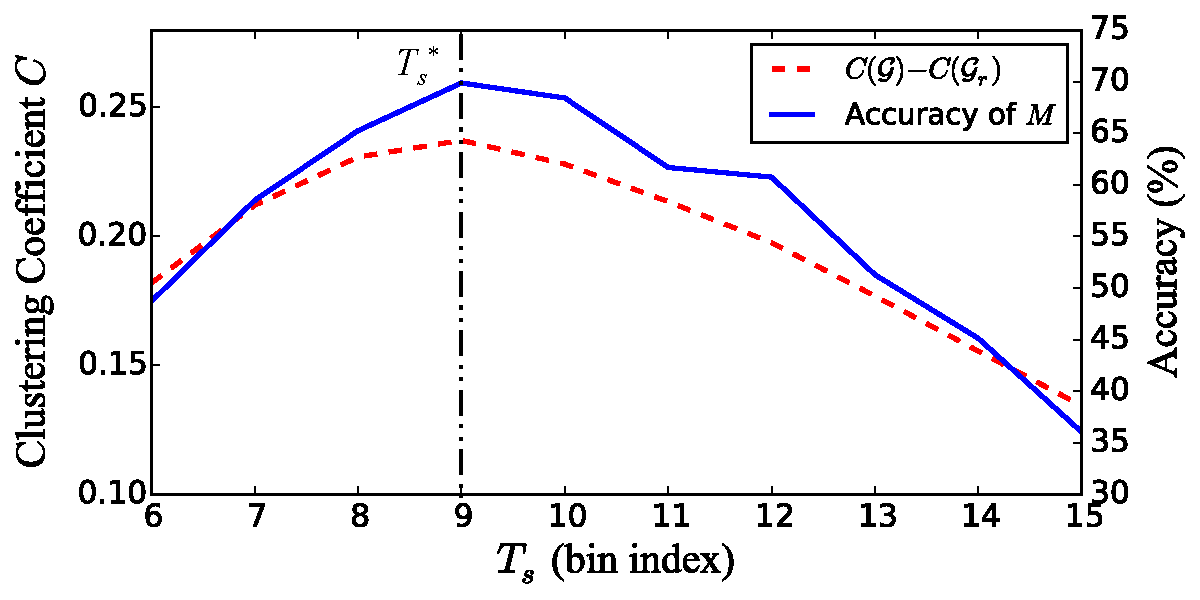
\includegraphics[width=.92\columnwidth]{figures/accuracy_Vs_thresold.pdf}
%	\end{center}
%	\caption{Accuracy of $M$ and $C(\mathcal{G})-C(\mathcal{G}_r)$ for different similarity thresholds.}
%	\label{fig:performance_across_thresholds}
%\end{figure}
%
%\begin{figure}
%	\begin{center}
%		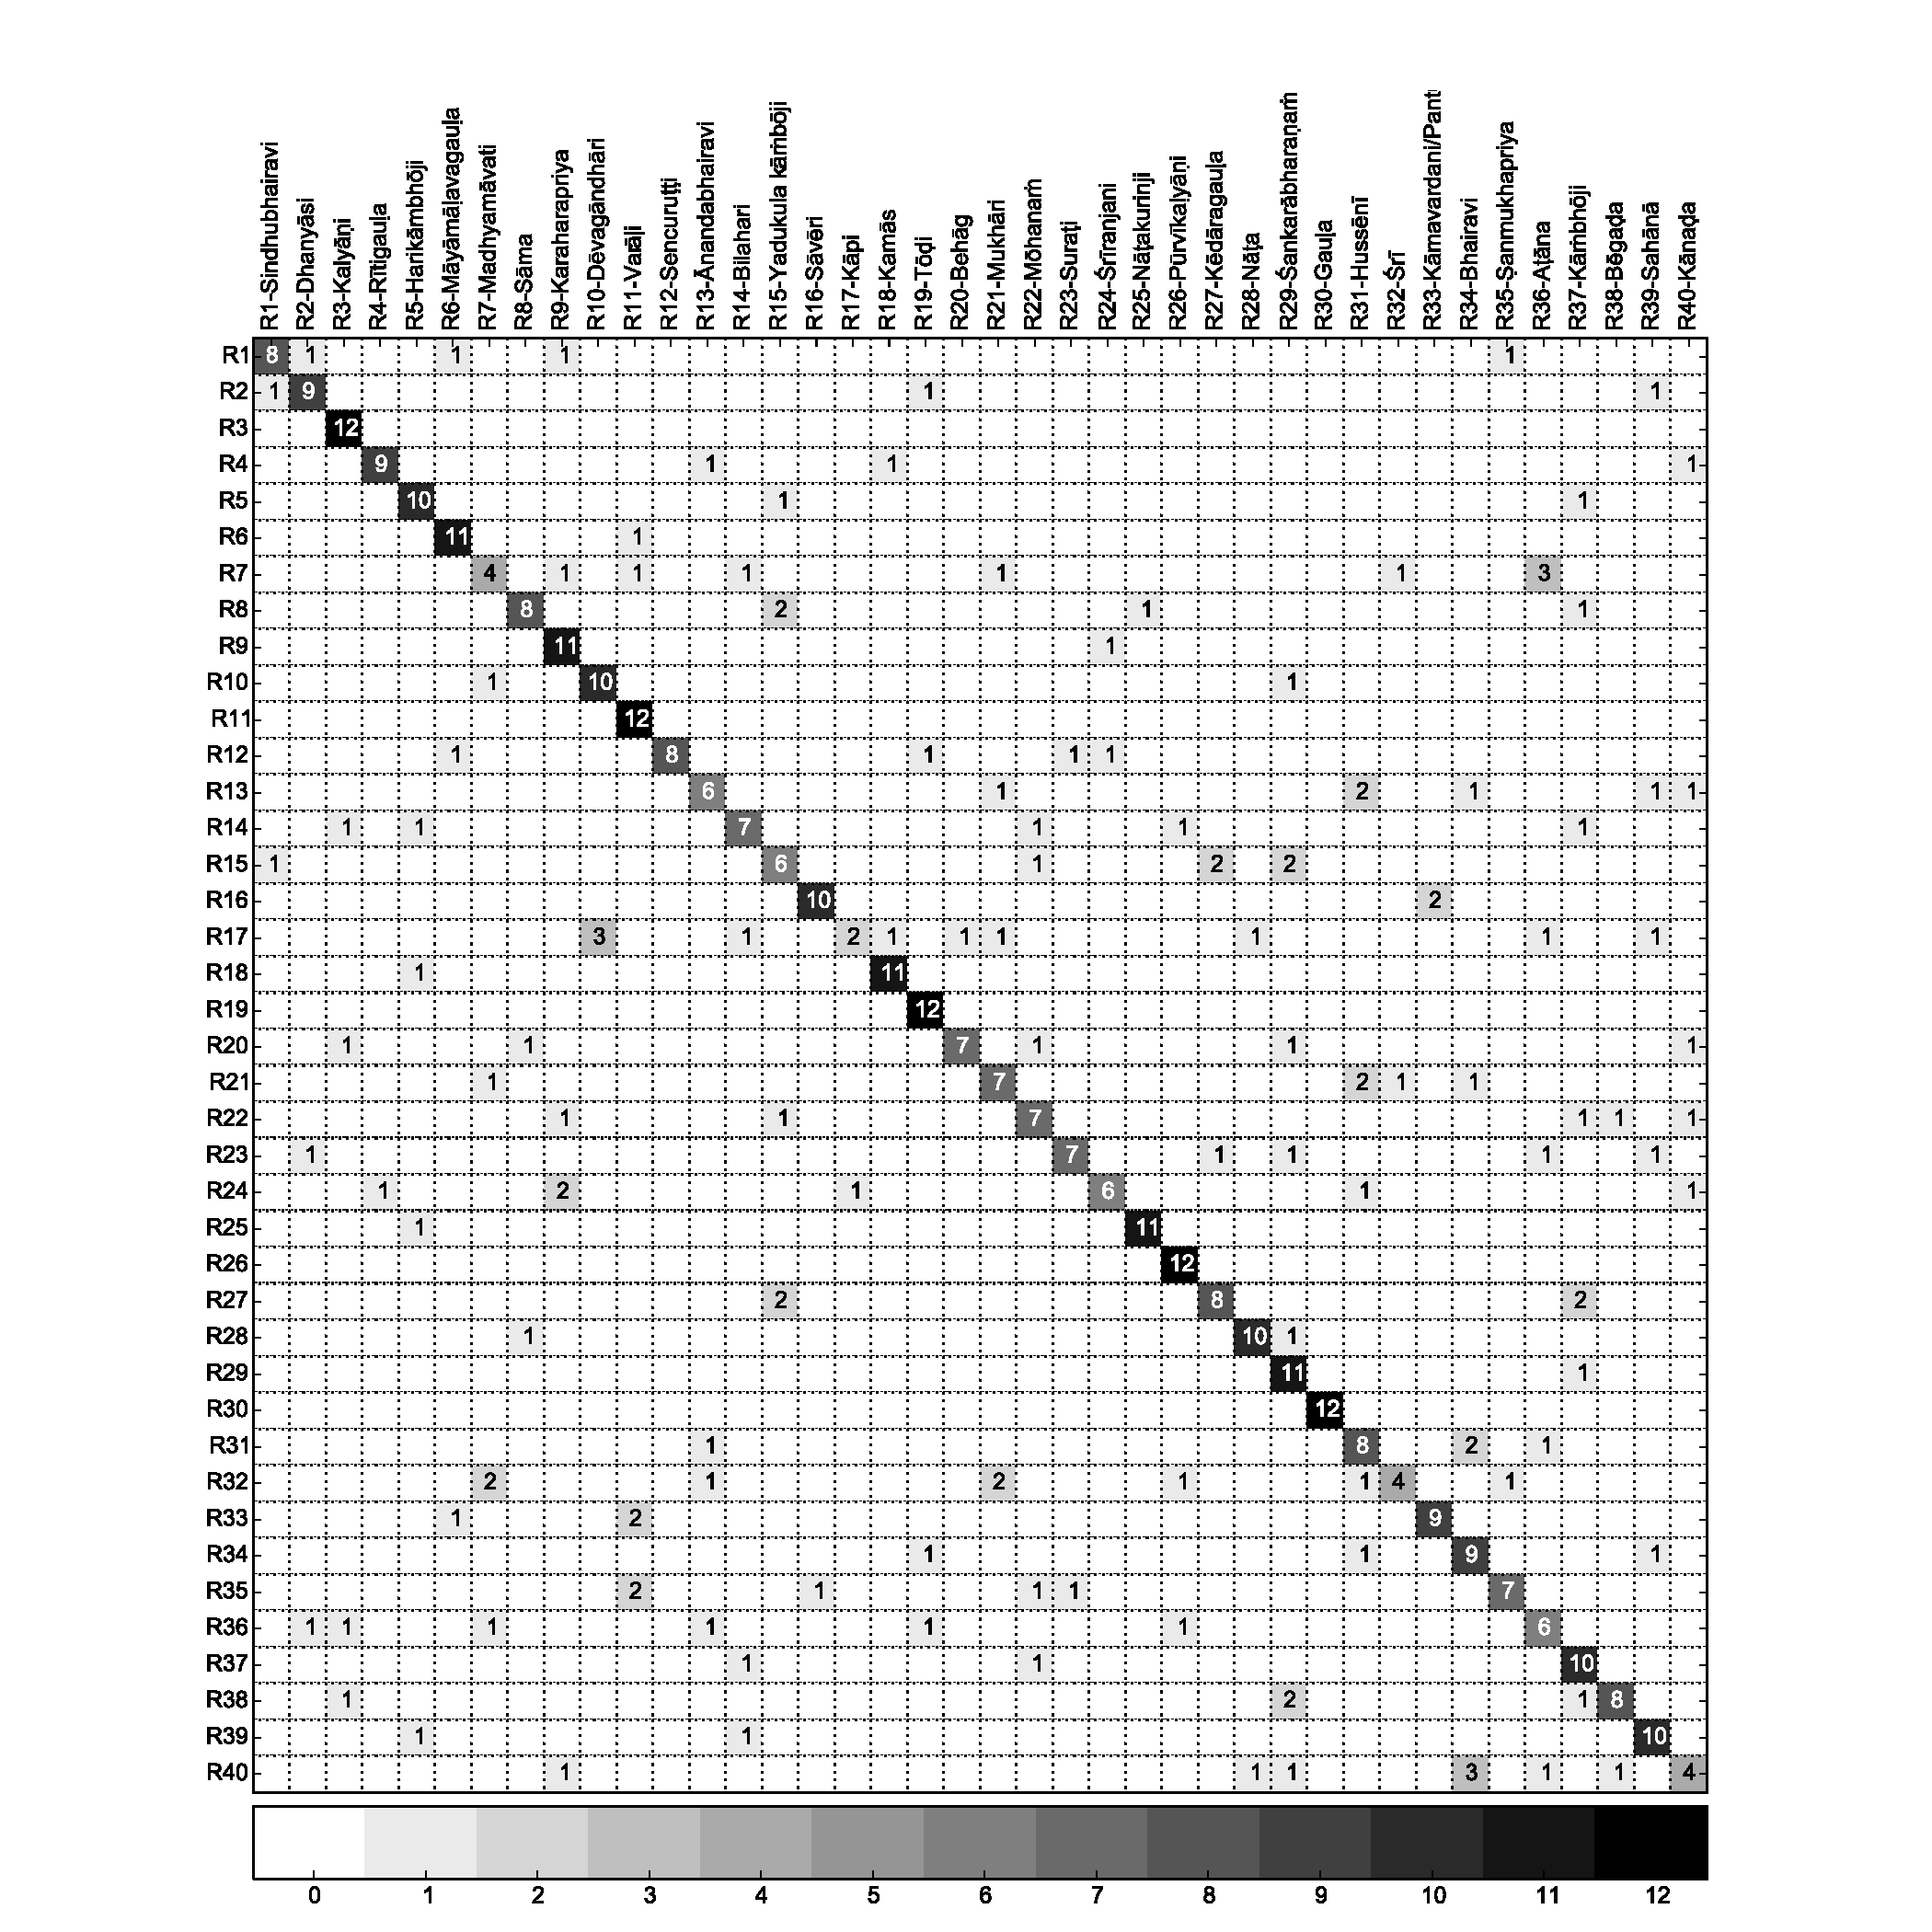
\includegraphics[width=\columnwidth]{figures/cnf_mtx_40raga_with_annotation.pdf}
%	\end{center}
%	\caption{Confusion matrix for the proposed method. The different shades of grey are mapped to different number of audio recordings.}
%	\label{fig:confusion_matrix}
%\end{figure}

Before further analyses of our results, we verify here our approach to obtain the optimal similarity threshold $T_{s}^\star$ (Section~\ref{pattern_clustering}). In Figure~\ref{fig:performance_across_thresholds}, we show the accuracy obtained by $M$, and  $C(\mathcal{G})-C(\mathcal{G}_r)$ as a function of similarity threshold $T_{s}$. We see that these curves are highly correlated. Thus, the optimal threshold $T_{s}^\star$, which we defined in Section~\ref{pattern_clustering} as the distance that maximizes the difference $C(\mathcal{G})-C(\mathcal{G}_r)$, also results in the best accuracy for r\={a}ga recognition.

We now analyze the confusion matrix, and understand the type of classification errors made by $M$, (Figure~\ref{fig:confusion_matrix}). We observe that our method achieves near-perfect accuracy for several r\={a}gas including Kaly\={a}\d{n}i, P\={u}rvikaly\={a}\d{n}i, T\={o}\d{d}i and Var\={a}\d{l}i. This is consistent with the fact that these are considered to be phrase-based r\={a}gas, that is, their identity is predominantly derived from melodic phraseology~\cite{krishna2012carnatic}. At the same time, we observe low accuracy for some other phrase-based r\={a}gas such as Madhyam\={a}vati, K\={a}na\d{d}a and \'{S}r\={i}. On investigating further we find that such r\={a}gas are confused often with their allied r\={a}gas\footnote{Allied r\={a}gas have a common set of svaras and similar melodic movement}~\cite{krishna2012carnatic}. Distinguishing between allied r\={a}gas is a challenging task, since it is based on subtle melodic nuances. We also note that, among the other r\={a}gas for which the obtained accuracy is low, several are considered as scale-based r\={a}gas. This is in line with~\cite{krishna2012carnatic}, where the authors remark that the identification of such r\={a}gas is not based on melodic phraseology. Overall, this analysis of the classification errors indicates that our proposed method is more suitable for recognizing phrase-based r\={a}gas compared to scale-based r\={a}gas. 


Finally, we compare $M$ with the state of the art methods $S_1$ and $S_2$. From Table~\ref{tab:accuracies_for_variants}, we see that $M$ outperforms $S_2$ for both the datasets, and the difference is found to be statistically significant. When compared with $S_1$, we see that $M$ performs significantly better than the $\mathrm{PCD}_{120}$ variant of $S_1$ for both the datasets. However, the performance of the $\mathrm{PCD}_{full}$ variant of $S_1$ is comparable to $M$ for DB10r\={a}ga, and, significantly better for DB40r\={a}ga. A comparison of the results of $M$ and $S_1$ for each r\={a}ga reveals that their performance is complementary. $M$ successfully recognizes several r\={a}gas with high accuracy for which $S_1$ performs poorly, and vice-versa. This suggests that the proposed phrase-based method can be combined with the pitch distribution-based methods to achieve a higher r\={a}ga recognition accuracy.



%
%1) What is the motivation behind this method, what can be its advantages
%2) What is the analogy that we have considered to devise the methodology


\section{\titlecap{\glsentrylong{tdms} for \glsentrytext{raga} recognition}}
\label{sec:tdms_raga_recognition}

\TODO{Rephrase intro to something impressive}

The approach described above for \gls{raga} recognition close to how humans identify \glspl{raga} and shows encouraging results. However, several challenges in reliably extracting melodic phrases and shortcomings summarized in Section~\TODO{ref} limit the performance of the system. In this section we propose a novel feature, the \gls{tdms}, that captures several melodic aspects that are useful in characterizing and distinguishing \glspl{raga}. \Glspl{tdms} alleviate some of the shortcomings mentioned above and improves the accuracy of \gls{raga} recognition by large margins. \Gls{tdms} is inspired by the concept of delay coordinates~\TODO{ref}. The main strengths of \gls{tdms} are:

\begin{itemize}
	\item It is a compact representation that describes both the tonal and the temporal characteristics of a melody
	\item It simultaneously captures the melodic characteristics at different time-scales, the overall usage of the pitch-classes in the entire recording, and the short-time temporal relation between individual pitches.
	\item It is robust to pitch octave errors.
	\item It does not require the transcription of the melody nor a discrete representation of it.
	\item It is easy to implement, fast to compute, and has a musically-meaningful interpretation.
	\item As it will be shown, it obtains unprecedented accuracies in the raga recognition task, outperforming the state-of-the-art by a large margin, without the use of any elaborated classification schema.
\end{itemize}


\subsection{\titlecap{\glsentrylong{tdms}}}
\label{sec:tdms_feature_extraction}

\begin{figure}
	\begin{center}
		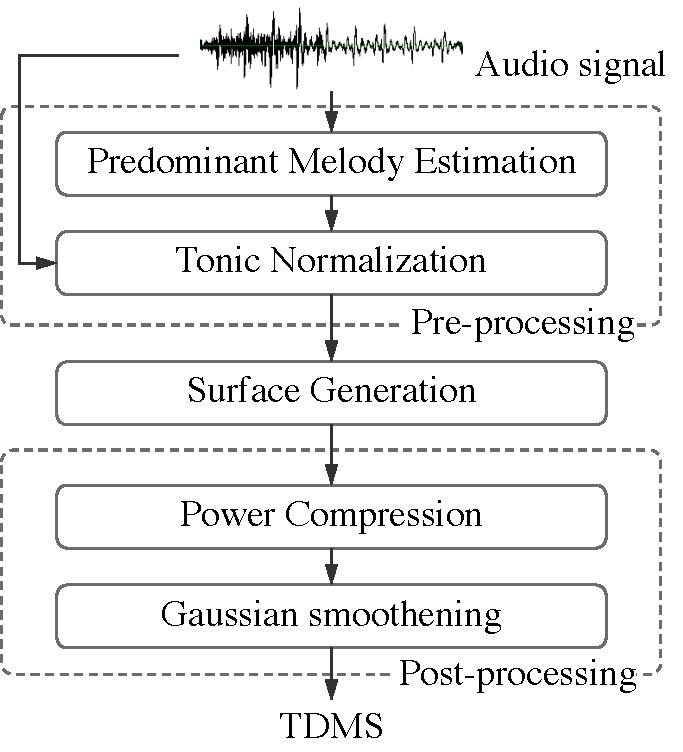
\includegraphics[width=\figSizeSixty]{ch07_ragaRecognition/figures/tdms_computation.pdf}
	\end{center}
	\caption{Block diagram for \gls{tdms} compuation}
	\label{fig:bd_tdms_computation}
\end{figure}

The computation of a \gls{tdms} has three steps as shown in Figure~\ref{fig:bd_tdms_computation}: pre-processing, surface generation, and post-processing. In pre-processing, we obtain a representation of the melody of an audio recording, which is normalized by the tonic or base frequency of the music piece. In surface generation, we compute a two dimensional surface based on the concept of delay coordinates. Finally, in post-processing, we apply power compression and Gaussian smoothing to the computed surface. We subsequently detail these steps.



\subsection{Classification and Evaluation Methodology}
\label{sec:tdms_classification_evaluation}

% Our second method  $\mathcal{M}_\mathrm{\acrshort{tdms}}$ uses a novel melodic representation, \gls{tdms}, for compactly capturing both the tonal and the temporal characteristics of \glspl{raga}. Evaluations done using representative and scalable data sets for both Hindustani and Carnatic music demonstrate that $\mathcal{M}_\mathrm{\acrshort{tdms}}$ outperforms state-of-the-art methods by a large margin. 
% 
%1) Motivation behind this method
%2) Desired qualities of this method


\subsection{Results and Discussion}
\label{sec:tdms_eval_results}

\section{Comparison with state of the art}
\label{sec:summary_raga_recognition}

\section{Summary}
\label{sec:summary_raga_recognition}




